\documentclass[11pt,a4paper]{article}
\usepackage[utf8]{inputenc}
\usepackage[T1]{fontenc}
\usepackage[spanish]{babel}
\usepackage{amsmath,amssymb}
\usepackage{booktabs}
\usepackage{graphicx}
\graphicspath{{../../matlab/}{./}}
\usepackage{geometry}
\geometry{margin=2.3cm}
\title{\textbf{Dise\~no del Controlador LQR para el P\'endulo Invertido sobre Dos Ruedas}\\
\large Procedimiento te\'orico y verificaci\'on en MATLAB}
\author{Proyecto de Control de Procesos}
\date{\today}

\begin{document}
\maketitle

\section{Modelo en espacio de estados}
El robot balanc\'in se modela como un p\'endulo invertido sobre dos ruedas. El
estado es $\mathbf{x}=[x,\ \dot{x},\ \theta,\ \dot{\theta}]^{\top}$ (posici\'on,
velocidad lineal, \'angulo y velocidad angular) y la entrada $u$ es el PWM del
motor. El modelo linealizado alrededor de la vertical es
\begin{equation}
\dot{\mathbf{x}} = A\mathbf{x} + Bu, \qquad y = C\mathbf{x},
\end{equation}
\begin{equation}
A=\begin{bmatrix} 0&1&0&0\\ 0&0&-7.4697&0\\ 0&0&0&1\\ 0&0&104.6806&0 \end{bmatrix},\quad
B=\begin{bmatrix} 0\\ 0.0316\\ 0\\ -0.2376 \end{bmatrix},\quad
C=\begin{bmatrix}1&0&0&0\\0&0&1&0\end{bmatrix}.
\end{equation}
El vector $B$ usa la ganancia de par \emph{real} del motor (calibrada en
hardware, $\approx 6\times$ menor que la nominal de placa). El polo inestable de
la planta es $s=+\sqrt{104.6806}=+10.23~\mathrm{rad/s}$: sin control, el robot cae.

\section{Controlabilidad}
La matriz de controlabilidad $\mathcal{C}=[B\ AB\ A^2B\ A^3B]$ tiene
$\operatorname{rank}(\mathcal{C})=4$, por lo que el sistema es \textbf{controlable}
y es posible ubicar los polos de lazo cerrado con realimentaci\'on de estado.

\section{Formulaci\'on del LQR}
El regulador \'optimo cuadr\'atico (LQR) minimiza el funcional de costo
\begin{equation}
J=\int_{0}^{\infty}\!\left(\mathbf{x}^{\top}Q\,\mathbf{x}+u^{\top}R\,u\right)dt,
\qquad Q=Q^{\top}\succeq 0,\ R=R^{\top}\succ 0.
\end{equation}
La ley de control \'optima es la realimentaci\'on de estado
\begin{equation}
u=-K\mathbf{x}, \qquad K=R^{-1}B^{\top}P,
\end{equation}
donde $P$ es la soluci\'on sim\'etrica definida positiva de la
\textbf{ecuaci\'on algebraica de Riccati} (ARE)
\begin{equation}
A^{\top}P+PA-PBR^{-1}B^{\top}P+Q=0.
\end{equation}
Las matrices $Q$ y $R$ son los \emph{par\'ametros de dise\~no}: $Q$ penaliza el
error de los estados y $R$ el esfuerzo de control. Su relaci\'on define el
compromiso desempe\~no/energ\'ia.

\section{Selecci\'on de $Q$ y $R$: regla de Bryson}
Para obtener un punto de partida sistem\'atico (y no puramente prueba y error) se
usa la \textbf{regla de Bryson}: cada peso es el inverso del cuadrado del
m\'aximo valor admisible de la variable correspondiente,
\begin{equation}
Q_{ii}=\frac{1}{x_{i,\max}^{2}}, \qquad R_{jj}=\frac{1}{u_{j,\max}^{2}}.
\end{equation}
As\'i, una variable con poco margen (m\'aximo peque\~no) recibe mayor peso. Los
m\'aximos f\'isicos elegidos para el robot son:

\begin{table}[h]\centering
\begin{tabular}{lccl}
\toprule
Variable & S\'imbolo & M\'aximo admisible & Peso \\
\midrule
Posici\'on        & $x_{\max}$        & 0.10~m      & $Q_{11}=100$ \\
Velocidad lineal  & $\dot{x}_{\max}$  & 0.5~m/s     & $Q_{22}=4$ \\
\'Angulo          & $\theta_{\max}$   & $10^\circ$=0.1745~rad & $Q_{33}=32.83$ \\
Vel. angular      & $\dot{\theta}_{\max}$ & $90^\circ$/s=1.571~rad/s & $Q_{44}=0.405$ \\
Control (PWM)     & $u_{\max}$        & 200               & $R=2.5\times10^{-5}$ \\
\bottomrule
\end{tabular}
\caption{M\'aximos admisibles y pesos por la regla de Bryson.}
\end{table}

\noindent Resultando
\begin{equation}
Q=\operatorname{diag}(100,\ 4,\ 32.83,\ 0.405), \qquad R=2.5\times10^{-5}.
\end{equation}

\section{C\'alculo de la ganancia $K$}
Resolviendo la ARE con estos $Q,R$ (funci\'on \texttt{lqr} de MATLAB) se obtiene
\begin{equation}
K=\begin{bmatrix} -2000.0 & -1319.8 & -2996.4 & -380.7 \end{bmatrix}.
\end{equation}

\section{An\'alisis del lazo cerrado}
Con $A_{cl}=A-BK$ los polos de lazo cerrado son
\begin{equation}
s=\{-34.60,\ -8.95,\ -2.57\pm 1.81j\}\ \mathrm{rad/s},
\end{equation}
todos en el semiplano izquierdo: el sistema es \textbf{estable}. Los polos
dominantes $-2.57\pm1.81j$ tienen $\omega_n=3.15~\mathrm{rad/s}$ y
$\zeta=0.82$ (bien amortiguado). La respuesta de recuperaci\'on desde una
inclinaci\'on inicial $\theta_0=$5^\circ$$ presenta:
\begin{center}
\begin{tabular}{lc}
\toprule
Sobrepaso (overshoot) & $32.6\%$ \\
Tiempo de asentamiento $t_s$ (2\%) & 1.71~s \\
Error en estado estacionario & $\approx 0$ \\
\bottomrule
\end{tabular}
\end{center}
(El sobrepaso corresponde a la oscilaci\'on de recuperaci\'on al lado opuesto,
propia de la din\'amica de 4\textsuperscript{o} orden.)

\begin{figure}[h]\centering
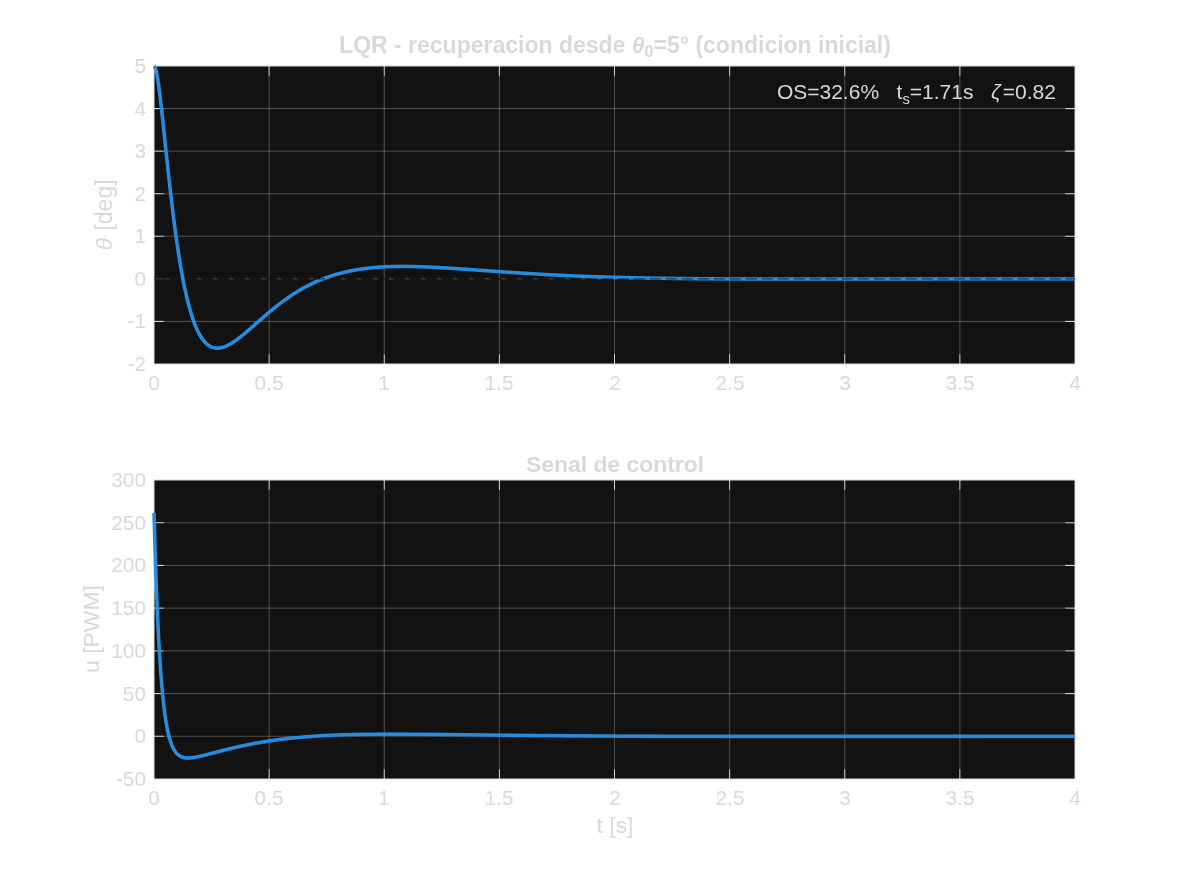
\includegraphics[width=0.75\textwidth]{lqr_diseno.png}
\caption{Verificaci\'on en MATLAB: recuperaci\'on de $\theta$ desde $5^\circ$ y se\~nal de control.}
\end{figure}

\section{Mapeo a las ganancias del firmware}
El firmware trabaja con $\theta$ en \emph{grados} y aplica
$u=K_{ang,p}\,\theta+K_{ang,d}\,\dot{\theta}$. La conversi\'on desde $K$ (en
radianes) es
\begin{equation}
K_{ang,p}=-K_3\cdot\frac{\pi}{180}=52.30~\tfrac{\mathrm{PWM}}{\mathrm{deg}},\qquad
K_{ang,d}=-K_4\cdot\frac{\pi}{180}=6.64~\tfrac{\mathrm{PWM}}{\mathrm{deg/s}}.
\end{equation}

\begin{table}[h]\centering
\begin{tabular}{lcc}
\toprule
Ganancia & Dise\~no LQR (te\'orico) & Hardware (sintonizado) \\
\midrule
$K_{ang,p}$ & 52.30 & 59.50 \\
$K_{ang,d}$ & 6.64  & 1.70 \\
\bottomrule
\end{tabular}
\caption{El dise\~no te\'orico coincide en orden de magnitud con el valor que
funciona en hardware ($K_{ang,p}$ a $\sim$12\%). $K_{ang,d}$ difiere porque en el
robot la derivada proviene directamente del giroscopio y se re-ajust\'o a mano.}
\end{table}

\section{Verificaci\'on en MATLAB}
Todo el procedimiento anterior se reproduce en el script
\texttt{matlab/lqr\_diseno.m}: construye $A,B,C,D$, aplica la regla de Bryson
para $Q,R$, resuelve la ARE con \texttt{lqr}, calcula polos, $\zeta$, sobrepaso y
$t_s$ mediante \texttt{initial}, y convierte $K$ a las ganancias del firmware.
Los valores num\'ericos de este documento coinciden con la salida del script.

\section{Conclusi\'on}
La regla de Bryson entrega un $Q,R$ inicial con sentido f\'isico que estabiliza
la planta inestable y logra un lazo cerrado bien amortiguado ($\zeta=0.82$). El
ajuste fino final se realiza por prueba y error sobre el robot, pero partiendo de
un dise\~no te\'orico que \emph{ya controla}, cercano a las ganancias medidas.

\end{document}
